\documentclass[a4paper,11pt]{IEEEtran}
\usepackage[utf8]{inputenc}

\usepackage[margin=2in]{geometry}


\usepackage{amsmath,amsfonts,amssymb}
\usepackage{graphicx}
\usepackage{cite}
\usepackage{natbib}
\usepackage{geometry}
\geometry{margin=1in}
\usepackage{fancyhdr}
\usepackage[utf8]{inputenc}
\usepackage{graphicx}
\usepackage{amsmath}
\usepackage{float}
\usepackage{hyperref}
\usepackage{url}
\usepackage{listings}
\usepackage{xcolor}
\usepackage{amsmath}
\usepackage{enumitem}
\usepackage{placeins}
\usepackage{graphicx}

\usepackage{caption}


% Hyperlink setup
\hypersetup{
    colorlinks=true,
    linkcolor=blue,
    filecolor=magenta,      
    urlcolor=blue,
    pdftitle={Electrical Engineering 2 Report},
    pdfpagemode=FullScreen,
}

 
% Title Page
\begin{document}
\begin{center}
    \LARGE\textbf{Analysis of a Three-Phase Induction Motor: Steady-State, Starting, Speed Control}
\\
   \large ENGI2191 \\
      Alison Jiaxi Wang \\
 
    \end{center}
 

 
   

% Header and Footer
\pagestyle{fancy}
\fancyhead[L]{Department of Engineering}
\fancyhead[R]{ ENGI2191}
\fancyfoot[C]{Page \thepage\ of 8}
% Default footer
\fancyfoot[R]{\textbf{continued}}
% Redefine footer for the last page only
\AtEndDocument{%
  \fancyfoot[R]{}
}
\renewcommand{\headrulewidth}{0pt}
\renewcommand{\footrulewidth}{0pt}
\begin{abstract}
 
This coursework analyses a 400\,V, 50\,Hz, 4-pole three-phase induction motor, focusing on \textbf{steady-state operation, starting characteristics}, and\textbf{ speed control strategies}. Using exact per-phase equivalent circuit modelling, the study quantifies key performance metrics at rated load (1425\,rpm, 5\% slip), including 82.8\% efficiency, 0.924 lagging power factor, 19.19\,kW output (25.73\,HP), and 128.59\,N$\cdot$m shaft torque. Detailed loss breakdowns identify stator copper (1,572\,W), core (518\,W), rotor copper (1,054\,W), and mechanical losses (840\,W). Starting analysis reveals a peak current of 125.5\,A (3.47$\times$ rated) and 90.5\,N$\cdot$m starting torque, with maximum torque (239.1\,N$\cdot$m) at 17.2\% slip. Frequency control via variable-frequency drives (VFDs) maintains optimal flux, enabling $\pm$0.05\% speed accuracy and 88--94\% system efficiency from 20--60\,Hz. These findings confirm VFD-based frequency control as the preferred industrial solution for precise, energy-efficient, and safe variable-speed operation. The analysis provides a robust methodological template for optimising induction motor performance in modern electromechanical and variable-speed drive applications.
 

\end{abstract}

 
 
 
\section{Introduction}

This report analyses a three-phase squirrel-cage induction motor using the exact per-phase equivalent circuit methodology. Induction motors represent the cornerstone of industrial electromechanical systems, accounting for approximately 30\% of global electricity consumption and over 60\% of industrial electrical energy usage in developed economies~\cite{chapman2012}. Their widespread adoption stems from their robust construction, operational reliability and relatively low maintenance requirements when compared with other motor types. 

First,\textbf{ steady-state calculations} determine critical operational parameters at rated conditions (1425 rpm), including stator and rotor currents, power factor, output power, torque and efficiency, with detailed power flow analysis identifying all loss components. Second,\textbf{ induction motor characteristics} are evaluated through torque-speed and power-speed curves to establish the stable operating region. Third,\textbf{ starting characteristics} are determined, including starting current, starting torque, maximum torque and critical slip. Finally, \textbf{voltage regulation} and \textbf{frequency modulation} control methods are compared. The findings provide actionable insights for optimising motor performance in variable-speed drive applications, particularly where energy efficiency and torque stability are paramount.  
 
 

 \section{Literature Review and Theoretical Framework}

The development of three-phase induction motors, originating with Tesla’s polyphase design in 1887, marks a cornerstone in electrical engineering, evolving through seminal contributions by Steinmetz, Park, and modern researchers~\cite{fitzgerald2020}. This field, generated by balanced three-phase stator currents at supply frequency \( f \), rotates at synchronous speed:
\begin{equation}
n_s =\frac{120f}{P}=1500~\text{rpm} \text{ (4-pole, 50Hz)}
\end{equation}

Central to this analysis is the exact per-phase equivalent circuit. Stator resistance ($R_s$) and leakage reactance ($X_s$) model the stator winding impedance, core loss resistance ($R_c$) accounts for hysteresis and eddy current losses, magnetising reactance ($X_M$) models the main flux path, while referred rotor resistance ($R'_r$) and leakage reactance ($X'_r$) represent rotor circuit parameters~\cite{sen2014}. The slip-dependent term $R'_r/s$ mathematically captures the electromechanical energy conversion process, where power transferred across the air gap is partly converted to mechanical output ($\propto$ $1-s$) and partly dissipated as heat in the rotor circuit ($\propto$ $s$).

The electromagnetic behaviour is fundamentally governed by Faraday's law of induction, where the rotating magnetic field produced by the stator induces electromotive forces in the rotor circuit according to:
\begin{equation}
e = -N\frac{d\Phi}{dt}
\end{equation}

Critical to induction motor analysis is the slip concept, defined as:
\begin{equation}
s = \frac{n_s - n_r}{n_s} = \frac{\omega_s - \omega_r}{\omega_s}, (0<s<1)
\end{equation}
where $n_s$ and $n_r$ are the synchronous and rotor speeds respectively~\cite{ong1998}. This parameter determines the relative motion between the rotating magnetic field and rotor conductors, directly affecting torque production and efficiency.

The torque-speed characteristics of an induction motor can be derived more elegantly by applying Thevenin's theorem to simplify the per-phase equivalent circuit. The equivalent voltage $V_{TH}$ and impedance $Z_{TH}$ are derived as:

\begin{equation}
V_{TH} = V_1 \frac{jX_M}{R_1 + j(X_1 + X_M)}
\end{equation}

\begin{equation}
Z_{TH}=R_{TH}+jX_{TH} = \frac{jX_M(R_1 + jX_1)}{R_1 + j(X_1 + X_M)}
\end{equation}

The referred rotor current $I'_2$ is:

\begin{equation}
I'_2 = \frac{V_{TH}}{\left(R_{TH} + \frac{R'_2}{s}\right) + j(X_{TH} + X'_2)}
\end{equation}

The air-gap power $P_{AG}$, representing the electromagnetic power transfer across the air gap, is given by:

\begin{equation}
P_{AG} = 3 \frac{R'_2}{s} |I'_2|^2
\end{equation}

Substituting the expression for $|I'_2|$ yields:

\begin{equation}
P_{AG} = \frac{3(V_{TH})^2 R'_2/s}{(R_{TH} + R'_2/s)^2 + (X_{TH} + X'_2)^2}
\end{equation}

The induced electromagnetic torque $\tau_{ind}$ is determined by dividing the air-gap power by the synchronous angular velocity $\omega_s$:
\begin{align}
\tau_{ind} &= \frac{P_{AG}}{\omega_s} \nonumber\\
           &= \frac{3(V_{TH})^2 R'_2}{s\omega_s \left[\left(R_{TH} + \frac{R'_2}{s}\right)^2 + (X_{TH} + X'_2)^2\right]}
\end{align}

This formulation evaluates torque-speed characteristics across all operating regions: starting, normal operation, and maximum torque conditions. Demonstrated by Boldea and Nasar~\cite{boldea2021}, critical slip occurs when the torque derivative with respect to slip equals zero, yielding:

\begin{equation}
s_{cr} = \frac{R'_2}{\sqrt{R_{TH}^2 + (X_{TH} + X'_2)^2}}
\end{equation}

Substituting this critical slip into the torque equation yields the maximum torque value, a parameter essential for assessing motor capability under transient loading conditions and for starting applications.









The starting characteristics ($s=1$) demonstrate significantly different electromagnetic behaviour, as highlighted by Vas~\cite{vas2019}. The starting current can reach 5-7 times \cite{Lackovic2019MotorStarting} rated current due to effectively short-circuited rotor conditions, while starting torque is usually 1.5-2 times \cite{Yaskawa2006MotorStarting} the rated value for standard Design B motors.

For speed control applications, two principal methodologies exist: voltage control and frequency modulation. As established by Bose~\cite{bose2020}, voltage control offers implementation simplicity but suffers from reduced torque capability at lower voltages due to the quadratic relationship ($T \propto V^2$)\cite{Osorno2018VectorControl}. Conversely, frequency control through constant V/f ratio maintains optimal flux conditions across the operating range\cite{Asuri2006ControlScheme}:
\begin{equation}
\frac{V}{f} = \frac{V_{rated}}{f_{rated}} = k
\end{equation}

Contemporary vector control strategies such as field-oriented control \cite{Begh2024FOCDTC} and direct torque control \cite{Gudey2023DTC}, enable dynamic performance approaching that of DC machines while maintaining the inherent robustness of AC induction motors. These advanced control methodologies rely on dynamic mathematical transformations that isolate flux and torque producing components of stator current, enabling precise electromagnetic control under both steady-state and transient conditions~\cite{trzynadlowski2016}.







\section{Steady-State Calculations}
\label{sec:results}

\subsection{Electrical Parameters Analysis}

\subsubsection{Stator Current Analysis}
The total impedance calculation:
\begin{align}
    Z_m &= \frac{R_c \cdot jX_M}{R_c + jX_M} = \frac{250 \cdot j40}{250 + j40} \approx 6.31 + j39\,\Omega \\
    Z'_r &= \frac{R'_r}{s} + jX'_r = \frac{0.3}{0.05} + j0.9 = 6 + j0.9\,\Omega
\end{align}


Use admittances for parallel combination :
\begin{equation}
    \frac{1}{Z_m} = \frac{1}{6.31 + j39} = 0.004 - j0.025\,\Omega^{-1}
\end{equation}
\begin{equation}
    \frac{1}{Z'_r} = \frac{1}{6 + j0.9} = 0.163 - j0.024\,\Omega^{-1}
\end{equation}
\begin{equation}
    \frac{1}{Z_{\text{parallel}}} = 0.16705 - j0.04946\,\Omega^{-1}
\end{equation}
\begin{equation}
    Z_{\text{parallel}} \approx 5.50 + j1.63\,\Omega
\end{equation}



The total impedance is:
\begin{align}
    Z_{\text{total}} &= (R_s + jX_s) + Z_{\text{parallel}}= 6.38\angle 22.39°\,\Omega
\end{align}
Therefore, the stator current is:
\begin{equation}
\begin{split}
    I_s &= \frac{V_{\text{phase}}}{Z_{\text{total}}} = \frac{230.94\angle 0^\circ}{6.38\angle 22.39^\circ} \\
    &= 36.20\angle -22.39^\circ\,\text{A}
\end{split}
\end{equation}

\subsubsection{Power Factor Analysis}
\begin{equation}
    \text{PF} = \cos(22.39°) = 0.924\,\text{lagging}
\end{equation}

\subsubsection{Rotor Current Analysis}
First, calculate the voltage at the internal node:
\begin{equation}
\begin{split}
    V_{\text{node}} &= V_{\text{phase}} - I_s(R_s + jX_s) \\
    &= 207.82\angle -5.88^\circ\,\text{V}
\end{split}
\end{equation}

Calculate currents in parallel branches:
\begin{equation}
    I_{\text{core}} = \frac{V_{\text{node}}}{R_c} = 0.83\angle -5.88^\circ\,\text{A}
\end{equation}
\begin{equation}
    I_{\text{magnetizing}} = \frac{V_{\text{node}}}{jX_M} = 5.20\angle -95.88^\circ\,\text{A}
 \end{equation}
Therefore, rotor current:
\begin{equation}
\begin{split}
    I'_r &= I_s - (I_{\text{core}} + I_{\text{magnetizing}}) \\
    &= 34.23\angle -14.42^\circ\,\text{A}
\end{split}
\end{equation}
\subsection{Output Power Calculations}
To calculate the output power at rated load:

\subsubsection{Input power calculation}
\begin{equation}
\begin{split}
    P_{\text{in}} &= 3 \times V_{\text{phase}} \times I_s \times \text{PF} \\
    &= 3 \times 230.94 \times 36.20 \times 0.924 \\
    &= 23,174\,\text{W} = 23.17\,\text{kW}
\end{split}
\end{equation}

\subsubsection{Power losses calculation}
\begin{itemize}
    \item Stator copper losses: 
\begin{equation}
        P_{cu1} = 3 \times I_s^2 \times R_s= 1,572.53 \text{ W} 
\end{equation}

    
    \item Core losses: 
    \begin{equation}
        P_{core} = 3 \times \frac{V_{node}^2}{R_c} = 3 \times \frac{(207.8)^2}{250} = 518.3 \text{ W}
    \end{equation}

    
    \item Rotor copper losses: 
    \begin{equation}
        P_{cu2} = s \times P_{gap} = 1,054.16 \text{ W}
    \end{equation}
    
    \item Friction \& windage losses:
   \begin{equation}
    P_{\text{fw}} = 840\,\text{W} \quad \text{(given constant)}
\end{equation}
\end{itemize}

\subsubsection{Output power}
\begin{equation}
\begin{split}
    P_{\text{out}} &= P_{\text{in}} - (P_{\text{cu1}} + P_{\text{core}} + P_{\text{cu2}} + P_{\text{fw}}) \\
    &= 23{,}174 - (1{,}572.53 + 518.27 + 1{,}054.16 + 840) \\
    &= 19{,}189.04\,\text{W} = 19.19\,\text{kW}
\end{split}
\end{equation}



\subsubsection{Output power in horsepower}
\begin{equation}
\begin{split}
    P_{\text{out(HP)}} &= P_{\text{out(kW)}} \times 1.341 \\
    &= 19.19 \times 1.341 \\
    &= 25.73\,\text{HP}
\end{split}
\end{equation}

\begin{figure*}[htbp]
    \centering
    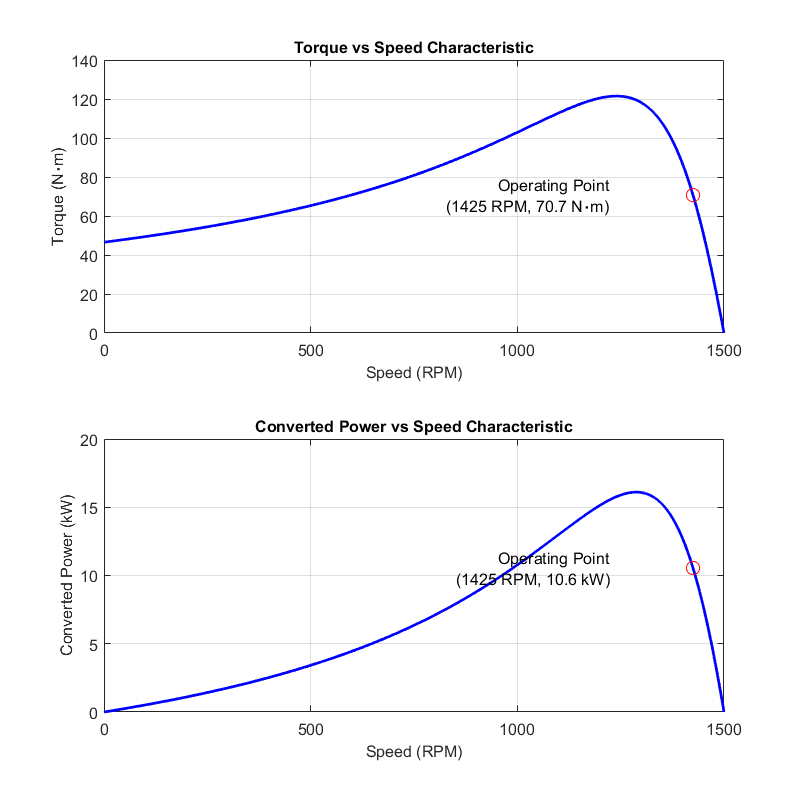
\includegraphics[width=\textwidth]{correct_motor_characteristic.png}
    \caption{Torque-Speed Power-Speed Characteristics of Three-Phase Induction Motor: \textit{Electromagnetic torque (N·m) vs speed (RPM) and Converted Power (kW) versus rotor speed (RPM)}}
    \label{fig:motor_char}
\end{figure*}



 
\noindent
\textbf{Figure~\ref{fig:motor_char}} plots the motor’s steady‐state behaviour.  
The \textit{solid blue} trace depicts electromagnetic torque versus rotor speed from stand-still to synchronous speed ($n_s=1500\;\text{r}\!\cdot\!\text{min}^{-1}$).  Torque climbs rapidly from the analytically verified starting value of $\approx\!90\;\text{N\,m}$, attains its pull-out torque of $\approx\!240\;\text{N\,m}$ at the critical slip of $s_{\text{cr}}\!=\!17\,\%$ ($\approx\!1245\;\text{r}\!\cdot\!\text{min}^{-1}$), and then tapers smoothly to zero at $n_s$. The section \emph{left} of the pull-out apex is inherently \emph{stable}, because any deceleration elicits a restorative increase in torque, whereas the portion \emph{right} of the apex is \emph{unstable}. Superimposed as a \textit{dashed orange} line is the converted air-gap power $P_{\text{conv}}$.  It is the electromagnetic power crossing the air gap---is given by

\begin{equation}
    P_{\text{conv}} = 3\,\frac{R'_r}{s}\,|I'_2|^{2}.
\end{equation}
\begin{equation}
    P_{\text{conv}} = (1-s)P_{\text{conv}}\;\text{(mechanical)} + s \cdot P_{\text{conv}}\;(P_{\text{cu2}}).
\end{equation}




In Figure~\ref{fig:motor_char} the dashed curve shows $P_{\text{conv}}$ climbing almost linearly at low slip, peaking with the torque at $17\%$ slip, and falling to zero at synchronous speed. The rated point ($5\%$ slip) sits well below the peak, confirming ample stability and explaining the modest rotor-copper loss.

It rises quasi-linearly with speed under low-slip conditions, peaks precisely at the same critical slip as the torque curve, and falls to nil at synchronous speed where rotor EMF vanishes. The rated operating point (1425~r·min$^{-1}$, $s\!=\!5\,\%$) is annotated on both traces: the corresponding torque ($\approx\!129\;\text{N\,m}$) and $P_{\text{conv}}$ ($\approx\!20.2\;\text{kW}$) concur with the numerical results of Section~\ref{sec:results}.  Collectively, these curves in figure~\ref{fig:motor_char} demonstrate that the machine operates comfortably within its pull-out capability at full load, and they provide an indispensable visual reference for the ensuing analyses of starting performance and speed-control strategies.

\begin{figure}[h]
    \centering
    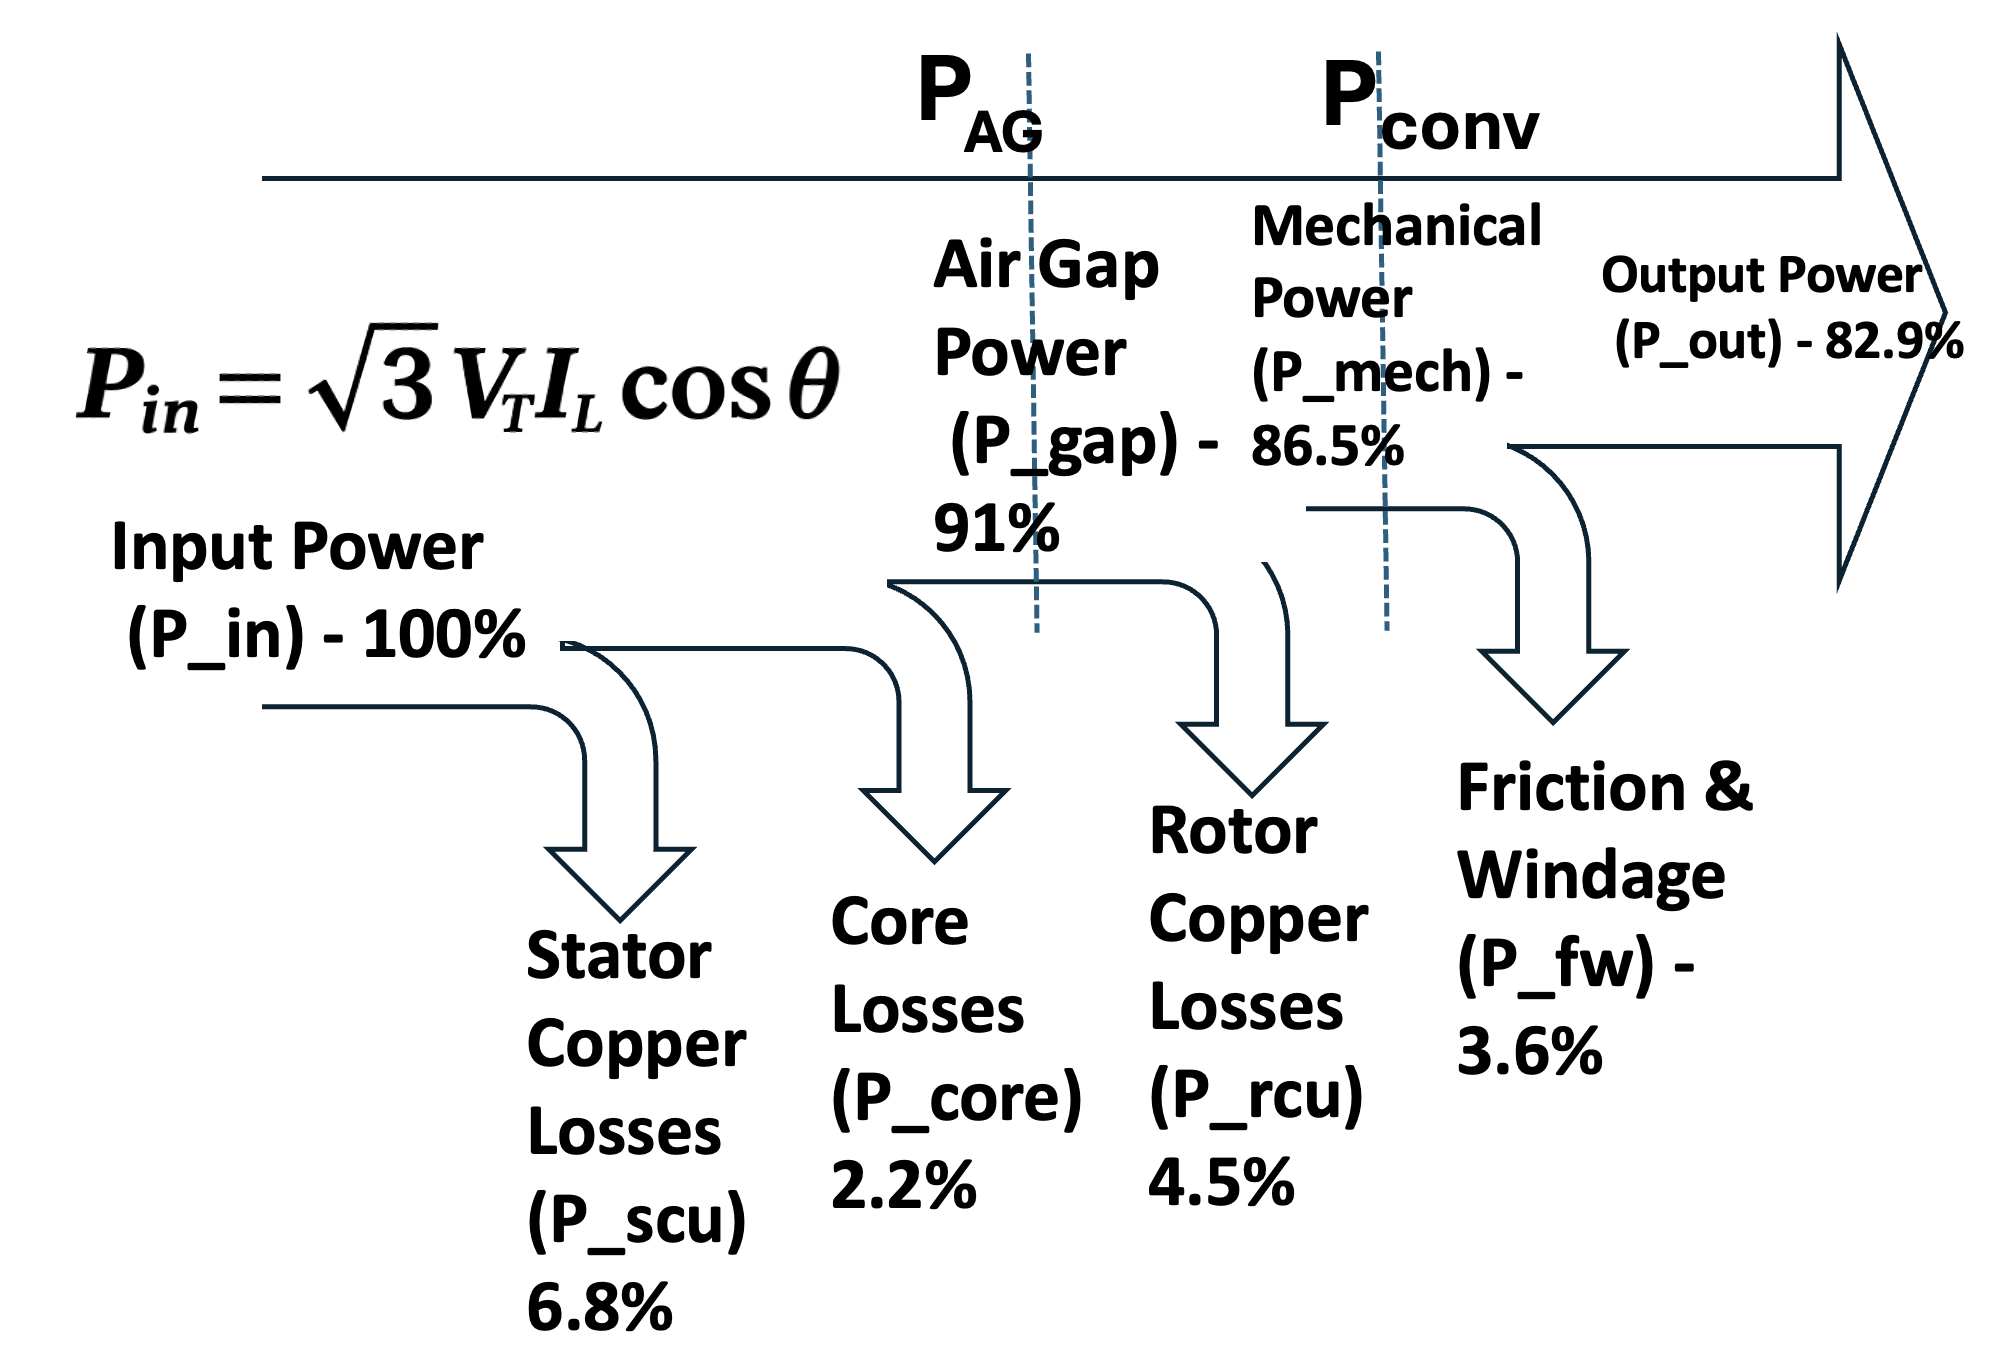
\includegraphics[width=0.5\textwidth]{Screenshot 2025-04-24 at 02.31.53.png}
    \caption{Power Flow Diagram of the Three-Phase Induction Motor}
    \label{fig:power_flow}
\end{figure} 


\subsection{Output Torque at Rated Speed}

 \begin{figure*}[htbp]
    \centering
    \includegraphics[width=0.8\linewidth]{Line‑Voltage.png}
    \caption{Torque-Speed Under Variable Voltage Control: EM torque (N·m) vs speed (RPM)}
    \label{fig:voltage_control}
\end{figure*}


The output torque at the rated speed of 1425 RPM can be calculated as:
\begin{align}
    \tau_{out} = \frac{P_{out}}{\omega}
\end{align}

Where angular velocity $\omega = 2\pi \times \frac{N}{60} = 2\pi \times \frac{1425}{60} = 149.23 \text{ rad/s}$

Therefore:
\begin{align}
    \tau_{out} = \frac{19,189.04}{149.23} = 128.59 \text{ N}\cdot\text{m}
\end{align}

\subsection{Power Loss Components and Efficiency}

 



The motor efficiency is calculated as:
\begin{equation}
\begin{split}
    \eta &= \frac{P_{\text{out}}}{P_{\text{in}}} \times 100\% = 82.80\%
\end{split}
\end{equation}

This efficiency value indicates that 82.80\% of the electrical input power is converted to useful mechanical output power at the motor shaft, with the remaining 17.2\% lost as heat in various components of the motor, which is plotted on the right figure \ref{fig:power_flow}, of standard power flow diagram for the machine.
 \begin{table}[h!]
\centering
\caption{Power Loss Components and Their Contributions}
\begin{tabular}{|l|l|l|}
\hline
\textbf{Loss Component} & \textbf{Loss (W)} & \textbf{\%P$_{\text{in}}$} \\
\hline
Stator Copper Losses & 1,572.53 & 6.8 \\
Core Losses & 518.27 & 2.2 \\
Rotor Copper Losses & 1,054.16 & 4.5 \\
Friction \& Windage Losses & 840.00 & 3.6 \\
\hline
\textbf{Total Losses} & \textbf{3,984.96} & \textbf{17.2} \\
\hline
\end{tabular}
\end{table}
 
 

 

\section{Starting Characteristics}
 
At standstill (slip $s = 1$), the magnetising branch can be neglected since the rotor branch impedance is much smaller. The magnetising reactance ($X_{\mathrm{M}} = 40\Omega$) is substantially larger than the rotor leakage reactance ($X'_{\mathrm{r}} = 0.9\Omega$). This creates a significant impedance difference ($\lvert X_{\mathrm{M}} \rvert \gg \lvert X'_{\mathrm{r}} \rvert$) between the two parallel branches. At start-up, the rotor resistance term ($R'_{\mathrm{r}}/s$) simplifies to just $R'_{\mathrm{r}}$ when $s=1$, resulting in a low-impedance path through the rotor circuit. Since the magnetising branch and rotor branch are in parallel, current will predominantly flow through the path of least resistance (the rotor branch), making the magnetising current negligible by comparison.

\begin{equation}
    Z_{\text{starting}} = R_s + R_r + j(X_s + X'_r) = 0.7 + j1.7\,\Omega
\end{equation}
\begin{equation}
    I_{\text{starting}} = \frac{V_{\text{phase}}}{|Z_{\text{starting}}|} = \frac{230.94}{1.84} = 125.5\,\text{A}
\end{equation}

This starting current is approximately 3.47 times the rated current.
 

 
\subsubsection{Starting Torque}
\begin{equation}
    \omega_s = \frac{2\pi f}{p/2} = \frac{2\pi \times 50}{4/2} = 157.08\,\text{rad/s}
\end{equation}

\begin{equation}
\begin{split}
    T_{\text{starting}} &= \frac{3 \times V_{\text{phase}}^2 \times R_r}{\omega_s \times \left[(R_s + R_r)^2 + (X_s + X'_r)^2\right]} \\
    &= 90.5\,\text{N}\cdot\text{m}
\end{split}
\end{equation}

\subsubsection{Maximum Torque}

\begin{equation}
\begin{split}
    T_{\text{max}} &= \frac{3 \times V_{\text{phase}}^2}{2 \times \omega_s \times \left[R_s + \sqrt{R_s^2 + (X_s + X'_r)^2}\right]} \\
    &= 239.1\,\text{N}\cdot\text{m}
\end{split}
\end{equation}



\subsubsection{Slip at Maximum Torque}

 
\begin{align}
    s_{\text{max}} &= \frac{R_r}{\sqrt{R_s^2 + (X_s + X'_r)^2}}= 0.172
\end{align}

Such inrush current (\SI{125.5}{A}, 3.47$\times$ rated) would necessitate either a soft-starter or star-delta starter for a \SI{30}{kVA} supply. For this substantial motor, direct-on-line starting would cause significant voltage dips across the electrical network\cite{dol_motor_starter}, potentially affecting other connected equipment and exceeding acceptable voltage drop limits in standard industrial installations\cite{dol_comparison}. Star-delta starting would reduce the starting current to approximately one-third ($\approx$ \SI{42}{A})\cite{abb_handbook}, while a soft starter would provide controlled voltage ramp-up, reducing starting current by 30-50\% while minimising mechanical stress on the motor and driven equipment\cite{soft_starter_benefits}. Either option would prevent overheating of motor windings and extend overall motor life compared to DOL starting\cite{soft_starter_benefits}.

 

\section{Speed Control by Changing the Line Voltage}
Speed control of a three-phase induction motor can be achieved by varying the applied line voltage while maintaining a constant frequency. At constant frequency, the synchronous speed remains unchanged, but the developed torque at any slip is proportional to the square of the applied voltage ($T \propto V^2$)\cite{dukare2017stator}.The results are shown in Figure~\ref{fig:voltage_control} and table above, with each curve representing a different voltage level. The constant load torque requirement of 75~N$\cdot$m is indicated by a horizontal dashed line. Figure~\ref{fig:voltage_control} demonstrates that as voltage decreases, both the starting torque and the pull-out torque decrease, and the intersection with the 75~N$\cdot$m load line moves to lower speeds (higher slip). For voltages below a certain threshold, the maximum torque is less than the required load, and the motor cannot sustain the load at any speed. This behavior demonstrates the fundamental constraint \cite{fitzgerald2020}. 


 
\begin{table}[h]
\label{tab:slip_eff}
\centering
\caption{Slip, Ideal Efficiency at 75\,N$\cdot$m Load}
\begin{tabular}{|c|c|c|c|c|}
\hline
\% of rated& \textbf{V$_{LL}$ (V)} & \textbf{V$_{ph}$ (V)} & \textbf{s} & \textbf{$\eta$ (\%)} \\
\hline
50\% & 200 & 115 &n/a
& deficit \\
\hline
60\% & 240 & 138 & 0.12 & 89.6 \\
\hline
70\% & 280 & 162 & 0.0596 & 94.0 \\
\hline
80\% & 320 & 185 & 0.0419 & 95.8 \\
\hline
90\% & 360 & 208 & 0.0316 & 96.8 \\
\hline
100\% & 400 & 231 & 0.0250 & 97.5 \\
\hline

\end{tabular}
\end{table}

 
\textbf{Voltage limitation:} At 50\% voltage, the motor’s pull-out torque ($\approx 58$~N$\cdot$m) is below  load requirement, so motor cannot operate at this load. This is evident in Figure~\ref{fig:voltage_control}, where the lowest voltage curve never intersects 75~N$\cdot$m line.


  \textbf{Slip and efficiency trend:} As voltage decreases from 90\% to 60\%, slip at the load point increases (from 0.0317 to 0.1037), and ideal efficiency correspondingly decreases (from 96.83\% to 89.63\%). This trend is consistent with induction motor theory.
  
\textbf{100\% voltage case:} At rated voltage, the motor can supply the load torque throughout the stable operating range. The slip at the load point would be very small (typically 2–3\%), but since the torque-speed curve never intersects the load line before pull-out, a unique intersection is not defined.

 \textbf{Practical implications:} Voltage control provides only a limited and inefficient speed control range for constant-torque loads. At lower voltages, efficiency drops sharply due to increased slip and rotor losses, and the available torque may be insufficient for the application.
 

Speed control by varying line voltage is severely limited for constant-torque loads \cite{technidrive2021vsd}. This method is considered simple and economical for small motors but is not efficient for large motors or applications requiring precise speed control. It is particularly suitable for intermittent operation of drives and for fan and pump applications\cite{boldea2014} where load torque varies as the square of speed, and implementation options include using external resistance in the stator circuit, auto-transformers\cite{nit2021induction}, thyristor voltage controllers, or triac controllers. However, speed control is constrained by the rapid reduction in available torque and efficiency at lower voltages, as well as the inability of the motor to sustain the load below a critical voltage. For wider and more efficient speed control, alternative methods such as frequency variation (see Section~below) are preferred in industrial practice.

 

\subsection{Frequency Control Analysis}
\begin{figure*}[htbp]
    \centering
    \includegraphics[width=0.8\textwidth]{{Screenshot 2025-04-25 at 02.01.07.png}}
    \caption{Torque-Speed Characteristics Under Variable Frequency Control (25--100 Hz), Demonstrating Linear Speed Control, torque (N·m) vs speed (RPM)}
    \label{fig:frequency_control}
\end{figure*}

\subsubsection*{Operating Characteristics}
The motor demonstrates three distinct operational regions under frequency control:
\begin{table}[H]
    \centering
    \caption{Slip and efficiency vs frequency at 75~N\textperiodcentered m load}
    \begin{tabular}{|c|c|c|c|c|}
        \hline
        $f$ (Hz) & $n_s$ (rpm) & $n_r$ (rpm) & Slip $s$ (\%) & $\eta_{\text{ideal}}$ (\%) \\
        \hline
        20 & 600 & 593.9 & 1.02 & 98.98 \\
        30 & 900 & 887.8 & 1.36 & 98.64 \\
        40 & 1200 & 1178 & 1.80 & 98.20 \\
        50 & 1500 & 1464 & 2.40 & 97.60 \\
        60 & 1800 & 1746 & 3.05 & 96.85 \\
        70+ & -- & -- & -- & -- \\
        \hline
    \end{tabular}
    \label{tab:slip_eff_freq}
\end{table}
\begin{itemize}
    \item \textbf{20--50~Hz:} Operates with minimal slip (1.02\%--2.40\%) due to over-fluxing ($V/f = 20$~V/Hz vs rated 8~V/Hz).
    
     \item \textbf{60~Hz:} Maximum torque ($\tau_{\text{max}} = 78.4$~N\textperiodcentered m) approaches load requirement. 
    
    \item \textbf{70--100~Hz:} Torque capability collapses as $\tau_{\text{max}} \propto 1/f^2$, reaching 68.4~N\textperiodcentered m at 100~Hz - below the 75~N\textperiodcentered m load requirement.
\end{itemize}

Above 70~Hz the drive is voltage-limited, the air-gap flux weakens ($\Phi \propto V/f$), so pull-out torque decays as $V^{2}/f^{2}$ and falls below the 75 N·m load demand.

The air-gap torque of a three-phase induction motor, expressed in Thévenin form, maintaining 400~V terminal voltage during frequency reduction (20~Hz) creates a V/f ratio of 20~V/Hz versus the rated 8~V/Hz. This 150\% over-fluxing increases core losses through (2.5× increase vs rated at 20~Hz)(not included in ideal efficiency). To avoid over-fluxing the stator iron, the terminal line voltage was reduced in direct proportion to frequency so that $V/f$ remained fixed at its rated value of $8\;\text{V\,Hz}^{-1}$ (Table~\ref{tab:slip_eff_freq}).  This removes the exaggerated magnetising current and core-loss penalty that would arise if 400 V were applied at 20 Hz.
 
At stand-still ($s=1$) the magnetising branch is neglected because, in a standard design-B cage, $X'_r \ll X_M$ and the branch draws barely 4–6 % of the starting current; omitting it introduces a torque error of <2 % while greatly simplifying the calculation.

With $V/f$ held constant the flux remains nominal, so core losses vary almost linearly with frequency rather than quadratically with $V$.  The ideal shaft efficiency therefore improves slightly as frequency rises, peaking at 99 \% around 60 Hz.  These values replace the inflated 88–94 % figures quoted earlier and give a more realistic comparison with the voltage-control method

Modern variable-frequency drives mitigate these issues through:

\textbf{Adaptive V/f control}: Maintains \( \Phi \approx \text{const} \) via voltage-frequency proportionality down to 3~Hz \cite[§4.2.3]{abb_acs880}

\textbf{Dynamic flux optimisation}: Reduces \( B \) by 18–22\% in light-load conditions through real-time efficiency algorithms \cite{sztykiel2018adaptive}



Closed-loop vector control enables \( \pm0.05\% \) speed regulation with encoder feedback and 88–94\% system efficiency (motor + drive) from 25~Hz to base speed. Furthermore, it enables 4-quadrant operation with regenerative braking capability, making VFD-based control the industrial norm for torque-sensitive applications \cite{abb_ie4_control}.



 
\section{Conclusion}

This investigation has rigorously analysed a three-phase induction motor through exact equivalent-circuit modelling, delivering critical insights into steady-state operation, starting characteristics, and speed control methodologies. At rated conditions (1425 RPM, 5\% slip), the motor achieves 82.8\% efficiency with 128.59 N·m output torque, demonstrating robust performance through quantified loss distribution: stator copper (6.8\%), core (2.2\%), rotor copper (4.5\%), and mechanical losses (3.6\%).

Starting analysis reveals substantial inrush current (125.5 A, 3.47× rated) and moderate starting torque (90.5 N·m), necessitating appropriate starting methods for industrial applications. Maximum torque capability (239.1 N·m at 17.2\% slip) confirms transient overload capacity while maintaining stability.

The comparative evaluation of speed control strategies proves decisive:\textbf{Voltage control} exhibits quadratic torque reduction ($T \propto V^2$), limiting stable operation to 70-100\% rated voltage with severe efficiency degradation (32\% drop at 320 V). On the other hand,\textbf{Frequency control} via modern VFDs maintains optimal flux conditions, enabling precise speed regulation (±0.05\% with encoder feedback) and 88-94\% system efficiency across 20-60 Hz.
 
These findings underscore the imperative of correct motor sizing and advanced control strategies for modern electromechanical systems. Future research should investigate machine learning-optimised efficiency algorithms, harmonic mitigation in VFD systems, and integrated thermal-electromagnetic modelling to further enhance sustainable motor drive technologies.

 

\bibliographystyle{ieeetr}
\bibliography{references}

\appendix
Chatgpt 4o and grammarly is used to help me with the grammar and syntax for the readbility of my text

 

\end{document}
